%\usepackage[parfill]{parskip}   
%
%\usepackage{bm}

%\section{}
%\subsection{}
%\chapter{}

%\begin{equation}...\end{equation}

%\begin{center}
%\end{center}

%\begin{itemize}
%\item blah blah
%\end{itemize}

%\begin{description}
%\item blah blah
%\end{description}

%\begin{enumerate}
%\item blah blah
%\end{enumerate}

%\begin{flushright}
%\end{flushright}

%\begin{figure}
%	\begin{center}
%		\includegraphics[scale=0.7]{nomdupdf}
%		\caption{Graphique}
%	\end{center}
%\end{figure}

%\listoffigures
%\listoftables

%\label{etiquette}
%\ref{etiquette}
%\pageref{etiquette}

%\begin{align*}
%A&=B\\
%&=C\\
%&=D
%\end{align*}

%\fbox


\newcommand{\fraction}[2]{\raisebox{0.5ex}{#1} \slash \raisebox{-0.5ex}{#2}}


\subsection*{Ice velocities using the stake positions of the previous year}

If we define each measured position of the mass balance stakes by $P_i(x,y,z)$ where $P$ accounts for the codename of the stake and $i$ labels the year of the considered stake, the horizontal distance $d$ between a stake $P_a(x_a, y_a, z_a)$ and $P_b(x_b, y_b, z_b)$ is given by :

\begin{equation}d = \sqrt{(x_a - x_b)^2 + (y_a - y_b)^2}\end{equation}

The horizontal surface velocity $u_s$ is calculated through :

\begin{center}
\boxed{u_s = \frac{d}{t_{a \rightarrow b}}}
\end{center}

where $t_{a \rightarrow b}$ is the elapsed time between the measurements $a$ and $b$.


\subsection*{Relating the surface velocity to depth-averaged ice velocity}

Now that we have the horizontal surface velocity, we wonder how it evolves with depth. Nye (1952 - REFERENCE) has proven that the overlying ice of a glacier must move at least as fast as that below. In quantitative terms, this translates to a reasoning that starts with the flow law for the strain rate $\dot{\epsilon}$ :

\begin{equation}\dot{\epsilon} = \left( \frac{\sigma}{B} \right)^n\end{equation}

with $\sigma$ a dominant shear stress, $B$ a viscosity parameter that increases with the stiffness of the ice, and $n$ the constant creep exponent. The latter has often experimentally proven to be $n \approx 3$, but for the sake of the derivation, we'll keep the value variable.
This law is also named after Glen's (1955 - REFERENCE), who conducted the first uniaxial compression experiments on ice.

We will follow up with the assumptions of the layer we consider being parallel-sided, that there's no flow in $y$ direction and that everything is uniform in $x$, $y$, as depicted in the \textsc{Figure} \ref{velocities}. The stress rate tensor therefore comes down to :


\begin{equation} \dot{\epsilon} = \left( \begin{array}{ccc}
0 & 0 & \dot{\epsilon}_{xz} \\
0 & 0 & 0 \\
\dot{\epsilon}_{zx} & 0 & 0
\end{array} \right) \end{equation}

From the constitutive relations, linking the stress $\sigma$ to the strain $\epsilon$ component per component, it follows that $\sigma_{xz} = \sigma_{zx}$ and hence :

\begin{equation}\dot{\epsilon}_{zx} = \left( \frac{\sigma_{zx}}{B} \right)^n\end{equation}


\begin{figure}
	\begin{center}
		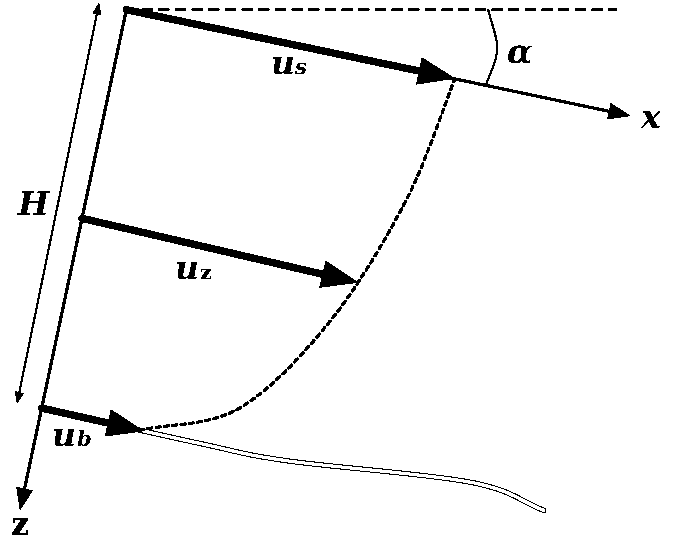
\includegraphics[scale=0.7]{VelocityProfile}
		\caption{Schematic diagram of our velocity profile}
		\label{velocities}
	\end{center}
\end{figure}

By the property $\dot{\epsilon}_{xy} = \frac{1}{2} \left( \frac{\partial u}{\partial y} + \frac{\partial v}{\partial x}\right)$, assuming the shear to take place in the plane normal to $z$ so that $\partial w / \partial x = 0$ and the stress configuration to be of simple shear, the last equation becomes :

\begin{equation}\frac{\mathrm{d} u}{\mathrm{d} z} = 2 \left( \frac{\sigma_{zx}}{B}\right)^n\end{equation}

We can express $\sigma_{zx}$ as a function of $z$ by using the coordinate system of \textsc{Figure} \ref{velocities} and noticing that $\sigma_{zx} = -\rho g h \sin{\alpha}$. After that, integration from the surface to the depth $z$ becomes possible :

\begin{equation}\int_{u_s}^{u(z)} \mathrm{d} u = -2 \left( \frac{\rho g \sin{\alpha}}{B}\right)^n \cdot \int_{0}^{z} z^n \mathrm{d} z\end{equation}


The depth-averaged ice velocity appears after carrying out the integration and rearranging the terms :

\begin{equation}u(z) = u_s - \frac{2}{n + 1} \left( \frac{\rho g \sin{\alpha}}{B}\right)^n \cdot z^{n+1}\end{equation}

This value becomes computable as soon as we know $u_s$, $B$ and $\alpha$. If we also know the total thickness $H$, the last equation becomes solvable at the bed and we get the bedrock velocity $u_b$ :

\begin{equation}u_b = u_s - \frac{2}{n + 1} \left( \frac{\rho g \sin{\alpha}}{B}\right)^n \cdot H^{n+1}\end{equation}

Our derivation here only is rigorously correct for a slab-shaped glacier of an infinite extent on a uniform slope. If for instance the glacier is bounded laterally, we will have to consider drag on the sides when calculating $\sigma_{zx}$ :

\begin{equation}\sigma_{zx} = -S_f \rho g z \sin{\alpha}\end{equation}

where we have introduced the shape factor $S_f$ ; we possess tables of values for different shapes, but it's good to remember that $S_f$ is $1$ for an infinitely wide glacier, and $\fraction{1}{2}$ for a semicircular glacier.

With that addition, our depth-averaged ice velocity finally reads :

\begin{center}
\boxed{u(z) = u_s - \frac{2}{n + 1} \left( \frac{S_f \rho g \sin{\alpha}}{B}\right)^n \cdot z^{n+1}}
\end{center}


\subsection*{The \textit{shallow ice} approximation and theory-motivated velocity}

This approximation concerns large ice sheets where conditions generally vary little over horizontal distances of 5-10 times the local ice thickness (Greve 2009 - REFERENCE). Ice flow then becomes determined by local conditions such as ice thickness, surface inclination and temperature.
In addition to this, we add some further assumptions :

\begin{itemize}
    \item our bedrock shall be \textit{flat} throughout our measurements
    \item the bedrock shall be frozen, and hence : $u_b = 0$
\end{itemize}

With this basis, the previously derived expression for the base velocity $u_b$ becomes :

\begin{equation}u_b = 0 = u_\circledS - \frac{2}{n + 1} \left( \frac{\rho g \sin{\alpha}}{B}\right)^n \cdot H^{n+1}
\quad
\stackrel{n = 3}{\Longrightarrow}
\quad
\boxed{u_\circledS = \frac{1}{2} \left( \frac{\rho g \sin{\alpha}}{B}\right)^3 \cdot H^4}\end{equation}

where $u_\circledS$ uses the circled subscript for the theory-motivated value of the ice velocity. We will keep using $u_s$ for the sake of generalization, but our theoretical computations in the next chapter will invoke this newly presented $u_\circledS$. 


\subsection*{Calculating the ice flux through an arbitrary cross section profile}

From definition, the ice flux per unit width $q$ is obtained by integrating the velocity profile over depth :

\begin{equation}q = \int_0^H u(z) \, \mathrm{d} z = u_s H - \frac{2}{(n+1)(n+2)} \left( \frac{S_f \rho g \sin{\alpha}}{B}\right)^n \cdot H^{n+2}\end{equation}

Introducing at this stage the mean velocity over depth $\bar{u} \equiv q/H$ reveals to be of greater advantage :

\begin{equation}\bar{u} = u_s - \frac{2}{(n+1)(n+2)} \left( \frac{S_f \rho g \sin{\alpha}}{B}\right)^n \cdot H^{n+1}\end{equation}

From here, after some calculus appears the very ergonomic expression :

\begin{equation}\bar{u} = \frac{4}{5}u_s + \frac{1}{5}u_b = \frac{4}{5}u_\circledS\end{equation}

This last expression allows us to jump back to a formula for the ice flux, reversing the definition of the mean velocity :

\begin{center}
\boxed{q = \bar{u}H = \frac{4}{5}u_\circledS H}
\end{center}


\subsection*{Mass balance and the \textit{steady state} assumption}

The massive ice flux per unit width can be defined through :

\begin{equation}q_m = \bar{\rho}q\end{equation}

where $\bar{\rho}$ is the vertically averaged density.

If we define an arbitrary planar cross-section $A$ of width $W$ around the positions where we measured $u_s$, and introduce the mass $M$ of the volume area comprised by $A \cdot H$, then the rate at which it changes would usually be defined (CUFFEY 2010 - REFERENCE) by :
 
\begin{equation}\left. \frac{\mathrm{d} M}{\mathrm{d}t} \right|_{\dot{b}_i} \equiv \bar{\rho} \int_A \dot{b}_i \, \mathrm{d}A - \int_W q_m \, \mathrm{d} W \end{equation}

where $\dot{b}_i$ is the ice-equivalent specific mass balance rate in $\left[ \fraction{m}{yr} \right]$.

But there is another way to measure the same rate, mainly by looking at the ice thickness through measurements of the surface and bed elevations, respectively $S$ and $B$. This gives us another approach to the mass changing rate :

\begin{equation}\left. \frac{\mathrm{d} M}{\mathrm{d}t} \right|_{S-B} \equiv \bar{\rho} \int_A (S-B) \, \mathrm{d}A\end{equation}

If the \textit{steady state} assumption happens to be true, then we'd have :

\begin{equation}\left. \frac{\mathrm{d} M}{\mathrm{d}t} \right|_{\dot{b}_i} \stackrel{\text{steady}}{=} \left. \frac{\mathrm{d} M}{\mathrm{d}t} \right|_{S-B}
\quad
\Leftrightarrow
\quad
\boxed{\dot{b}_i = S-B}
\end{equation}

This equality would reveal an extreme slow and hence negligible velocity flux in the glacier, and correlate this observation with our experimental values.